\section{Implementation}

\subsection{Smart contract}

The smart contract that I have implemented is written in Go. I coded it using the provided template of cothority, which is a generic smart contract that takes key-value pairs. My smart contract, that has been adapted to the situation, takes as inputs the URL of a web page and a CSS selector that can specify the page content that has to be certified (for example a specific paragraph of an article). The selected content must be deterministic, since each node will need to see the same content in order to reach a consensus. Thus, dynamic pages are excluded. The user can also specify if he wants the full HTML code or just the text of the chosen web page. Once the above specifications chosen, the smart contract saves the hash of the extracted content, the actual content, the URL, the selector, the current date and if the content consists of HTML code or if it is just the text on the skipchain.

The API I had to provide for this contract is constituted of three methods, namely \texttt{spawn}, \texttt{invoke} and \texttt{delete}. To spawn an instance of a smart contract means to create one. The method \texttt{invoke} is useful to update an already existing smart contract instance. I thought it was not relevant in this situation, as the goal of this project is to conserve the content of a web page at some point in time, and there is no need to further update the content of an instance. If a user wants to certify the same web page later, spawning another instance seems more logical to me, because even if the two instances refer to the same website, the content may not be the same. Thus, both of these instances are useful. This is why I have not implemented this method. Finally, a smart contract instance can also be deleted. However, even though this method is implemented, it is not present in the plugin because it not a feature that is particularly relevant. 

In order to extract only some specific section of a web page, CSS selectors have been used to indicate what to save on the skipchain. To use the passed selector, the library \texttt{goquery}\cite{goquery} has been used.

The hash function chosen is BLAKE2b \cite{Blake2bpaper}. For the smart contract written in Go, the package \texttt{blake2b} \cite{cryptoblake2b} has been used and for the plugin (that is described in the next section), the library used is named \texttt{blakejs} \cite{blakejs}. Both libraries implemented the BLAKE2b hash algorithm defined by RFC 7693 \cite{ietf}. Also, to randomize the hashes, namely to avoid that a same content leads to the same hash, I concatenated the creation date to the content and then hashed this. This could be improved since a same content that is certified on the same day will still lead to the same hash value, but this is a start.

\subsection{Browser plugin}
The browser plugin has been developed as a Chrome extension because I am familiar with Chromium since it is the browser I use. This extension is written in Typescript because the types are assisted, unlike in JavaScript. Webpack has been used as the bundler, and Babel as the ES6 transpiler. The file \texttt{webpack.config.js} at the root of the plugin is telling Webpack to start from the file \texttt{src/popup.ts} and look for TypeScript and JavaScript files. Typescript files are transpiled to ES6, while ES6 files are transpiled to ES5 with Babel. After this, everything is bundled in the \texttt{dist/bundle.min.js}. The plugin allows the user to invoke the smart contract described above when he is consulting a web page and wants to certify it. Its features are made to be easily found and understood as it can be seen in Figure \ref{f1}.

\begin{figure}[H]
    \centering
    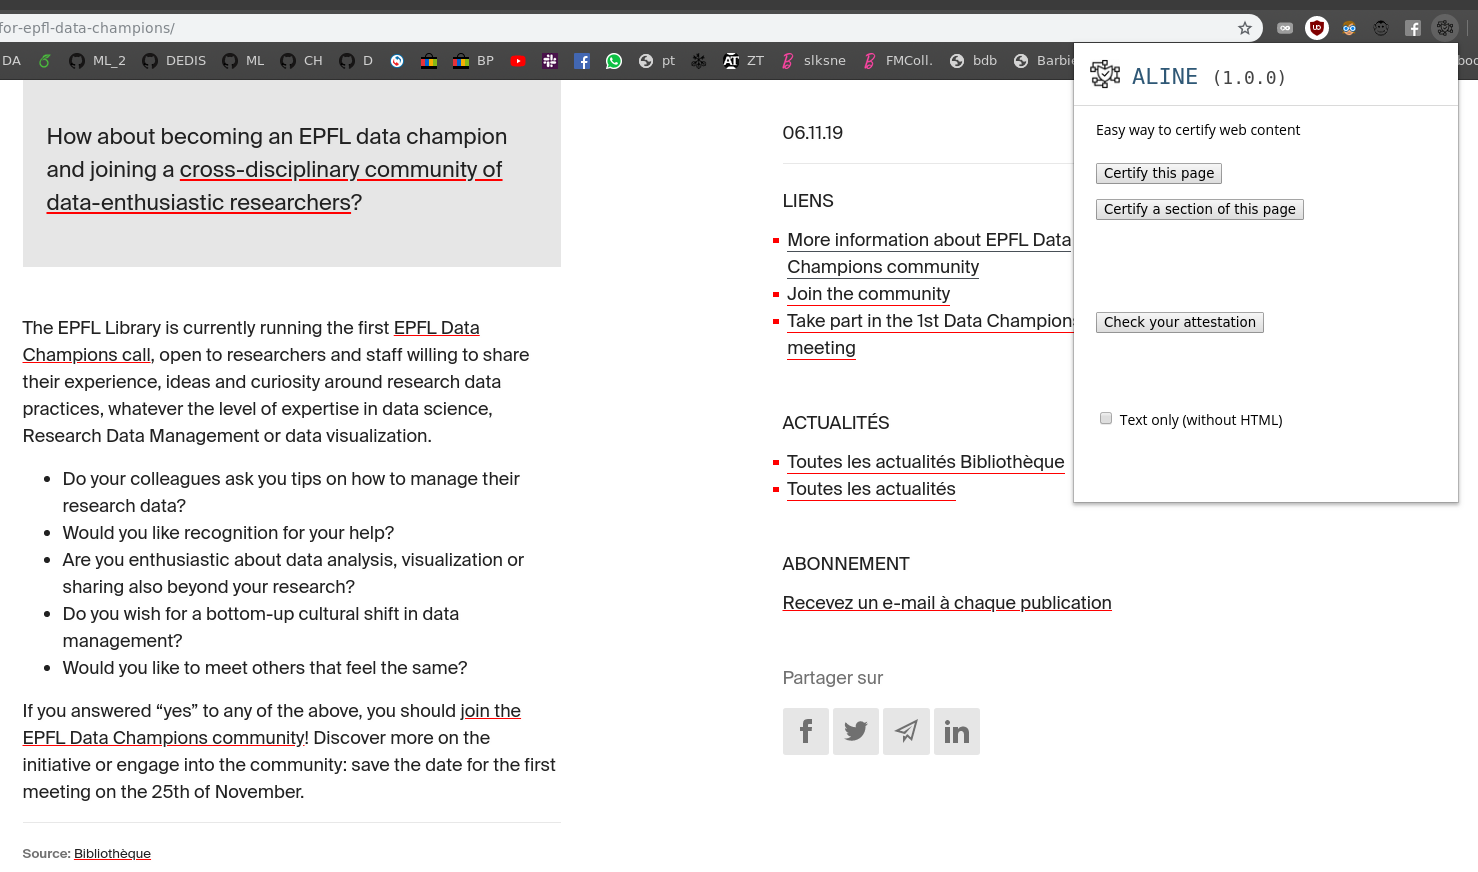
\includegraphics[width=1\linewidth, frame]{images/ALINE_presentation.png}
    \caption{Aline Chrome extension}
    \label{f1}
\end{figure}

It connects to the cothority and sends the current URL with the CSS selector and the Boolean value of a check-box which indicates if the user wants the text only or the full HTML code. In Figure \ref{f2}, we can see that the Chrome extension is currently creating the attestation.

\begin{figure}[H]
    \centering
    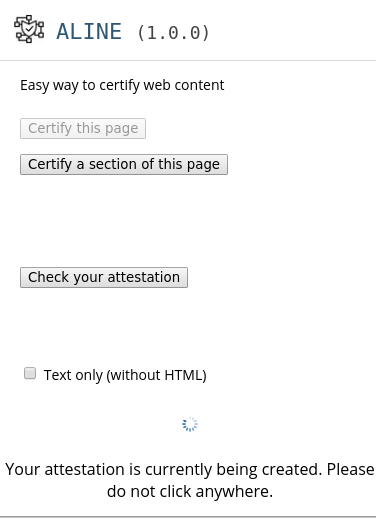
\includegraphics[width=0.4\linewidth, frame]{images/attest_currently_created.png}
    \caption{The attestation is currently being created}
    \label{f2}
\end{figure}

If the cothority reaches a consensus, the hash value and the other attributes are saved on the cothority ledger. If the user only wants to certify a section of the web page, he can interactively select it as it can be observable in Figure \ref{f3}. In my opinion, this is an important feature to provide since the average type of user will not know anything about CSS selectors. Thus, allowing him to choose what to certify in an intuitive way seemed indispensable. To do so, I used a module  called "Selector Gadget" \cite{selectorgadget} that can be called on the current web page we are consulting. To use it in the context of my Chrome extension, I had to code various scripts that would call Selector Gadget when it was relevant for the user. Once the page section chosen, the attestation can be generated. Figure \ref{f4} shows the screen the user sees when its attestation has been successfully created.

\begin{figure}[H]
    \centering
    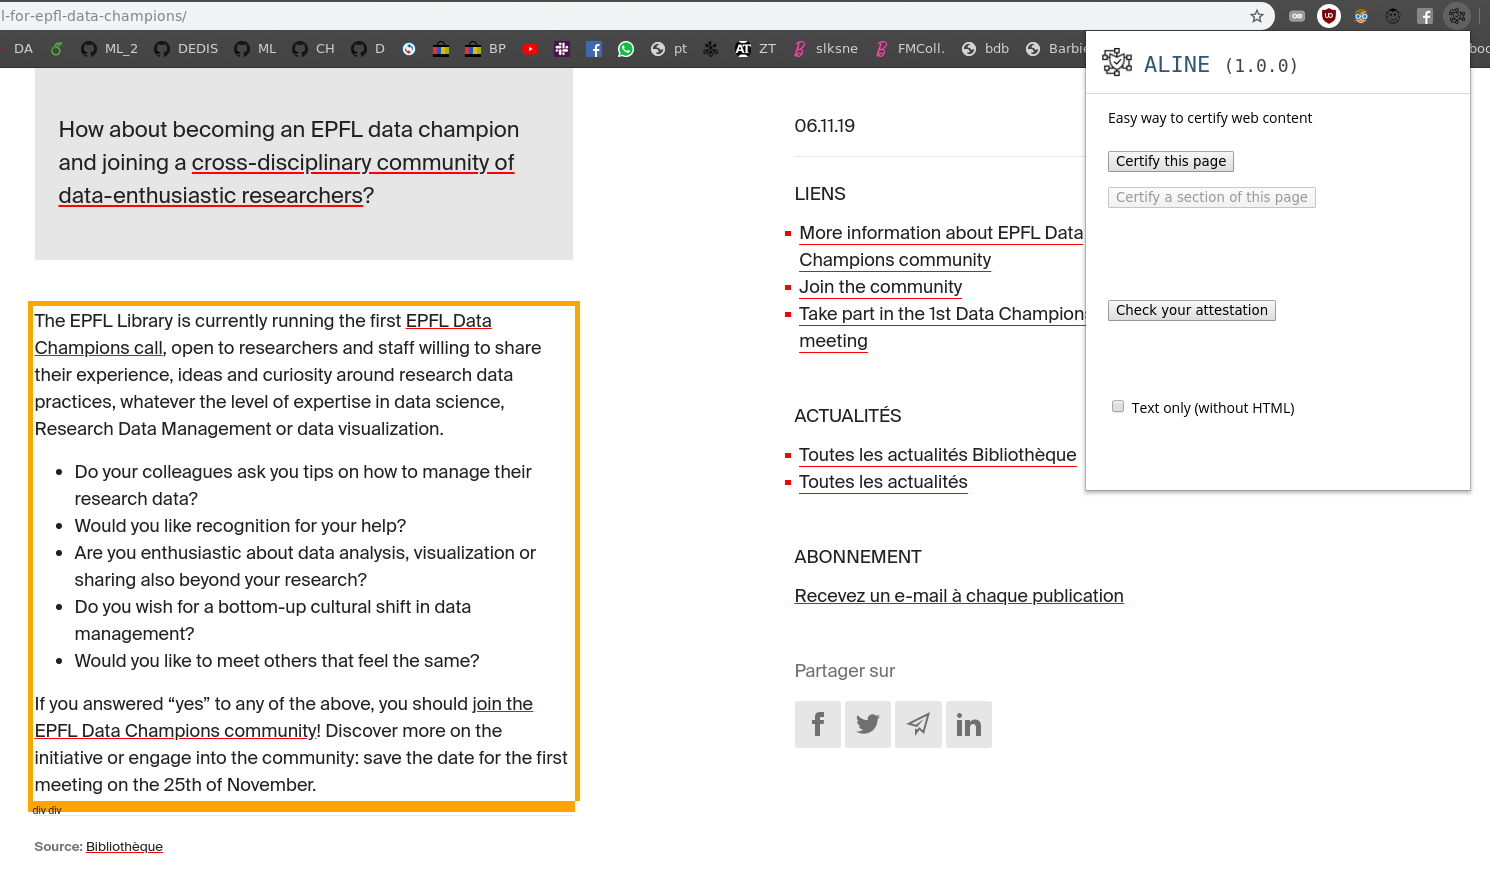
\includegraphics[width=1\linewidth, frame]{images/selector_gadget.png}
    \caption{The user can interactively select only a section of the page if needed}
    \label{f3}
\end{figure}

\begin{figure}[H]
    \centering
    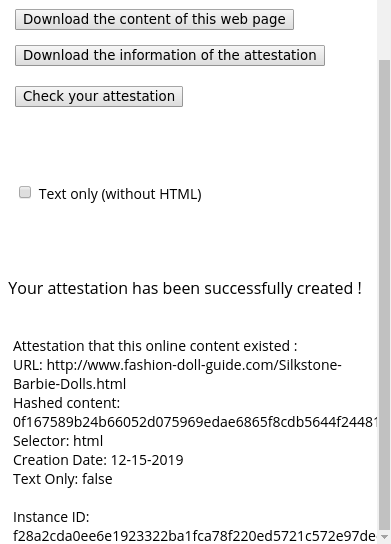
\includegraphics[width=0.4\linewidth, frame]{images/attest_successfully_created.png}
    \caption{The attestation has been successfully created}
    \label{f4}
\end{figure}

Once the attestation has been created by spawning a new instance of the web page smart contract, the user can download the information of the attestation as well as the content of the certified web page.

The user can then provide the instance ID and the content to anyone and prove the existence of this content. The extension indeed allows users to check the content of an attestation as we can notice in Figure \ref{f5}. By providing the smart contract's instance ID of the certificate and its content, the plugin will hash the provided content and compare it with the one stored on the skipchain at the given instance ID. We can see that the plugin will output a green tick if the check was successful (please refer to Figure \ref{f6}), or a red cross otherwise. This is useful because the user can send the content of the web page along with the ID and the person that needs to be convinced can use the plugin to check that it indeed holds. If the ID is not valid, ALINE let the user know it as shown in Figure \ref{f7}. This procedure is illustrated in Figure \ref{fb}.

\begin{figure}[H]
    \centering
    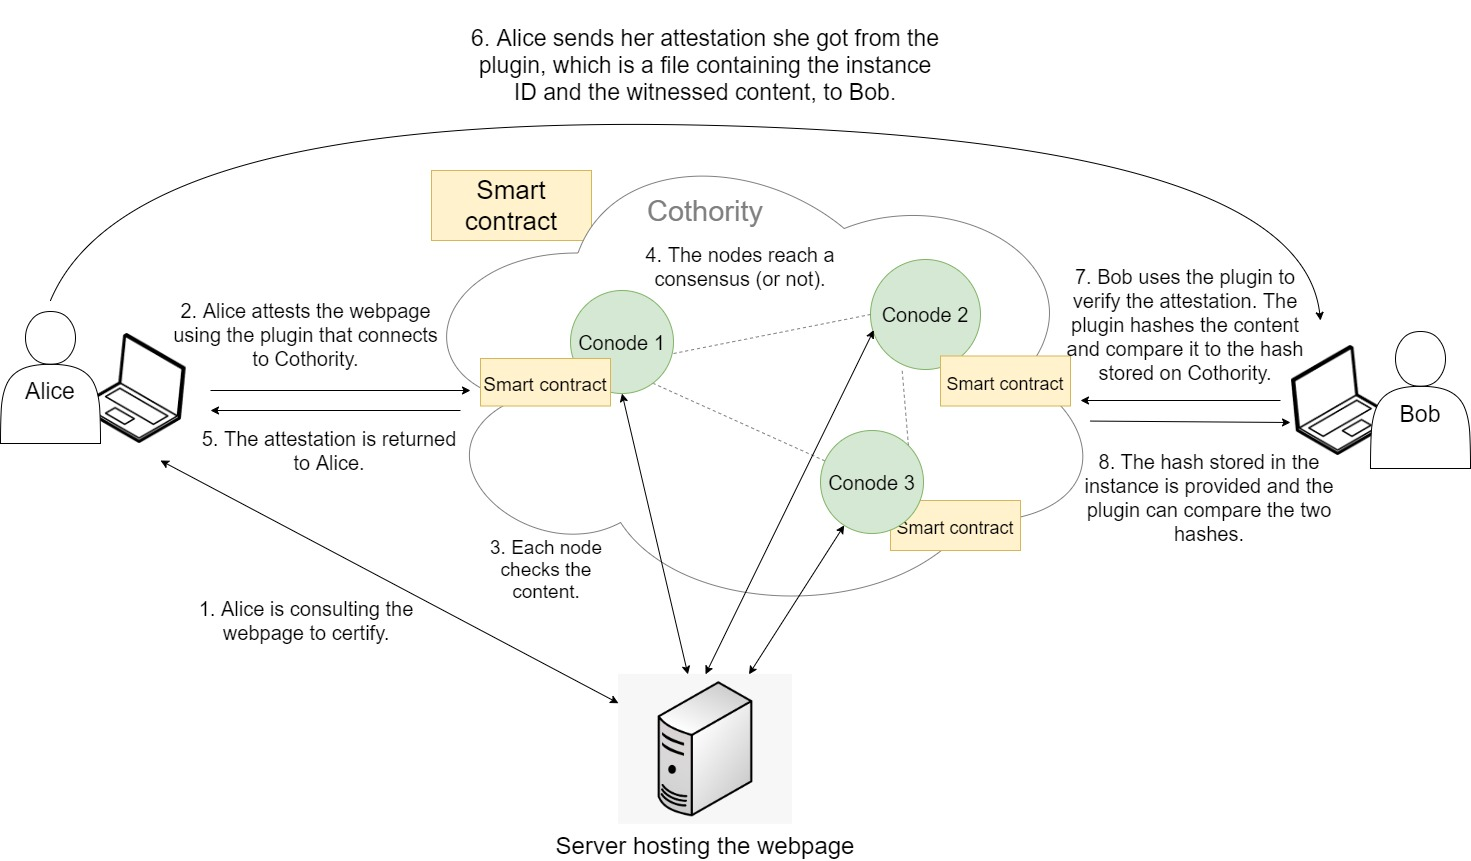
\includegraphics[width=1\linewidth]{images/Bob.jpg}
    \caption{ }
    \label{fb}
\end{figure}

\begin{figure}[H]
    \centering
    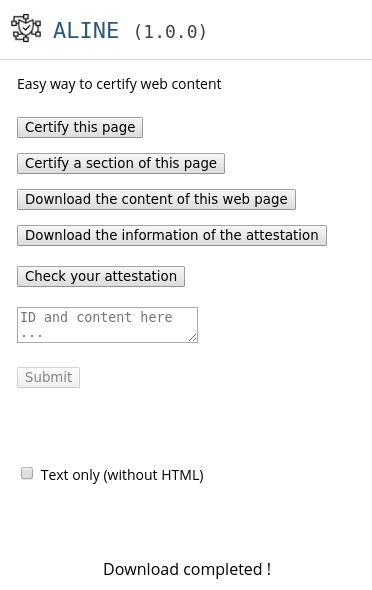
\includegraphics[width=0.4\linewidth, frame]{images/check_presentation.png}
    \caption{The content can be attested at any time after its creation}
    \label{f5}
\end{figure}

\begin{figure}[H]
    \centering
    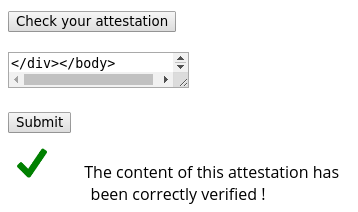
\includegraphics[width=0.4\linewidth, frame]{images/check_verified.png}
    \caption{Here is an example of a content that has been verified}
    \label{f6}
\end{figure}

\begin{figure}[H]
    \centering
    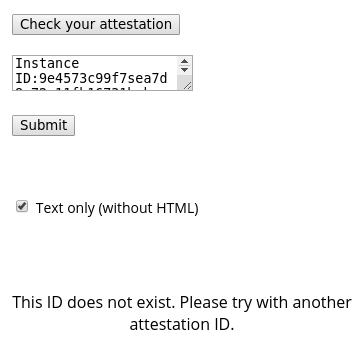
\includegraphics[width=0.4\linewidth, frame]{images/check_ID_error.png}
    \caption{The user has not a valid ID and is informed of it}
    \label{f7}
\end{figure}

